\chapter{Results and discussion}
\label{chap:results}

\section{Characteristics of q\textsubscript{1} - q\textsubscript{2} stability diagrams for one electron}

%\subsection{Comparison of simulation and determinant stability criterion}

We will start by looking at the stability diagrams for different $\nicefrac{\Omega_2}{\Omega_1}$ ratios. Starting with \ref{fig:stabil-eta=3}.

\begin{figure}[H]
\begin{subfigure}{.5\textwidth}
  \centering
  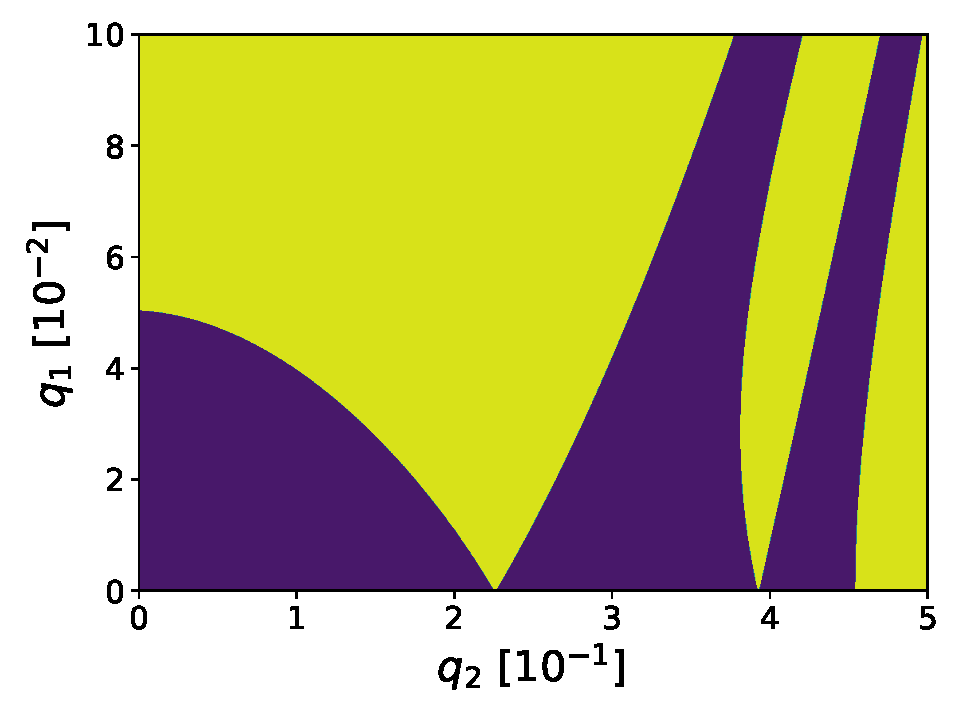
\includegraphics[width=\linewidth]{img/det_q1_0.0-0.1_q2_0.0-0.5_990x990_3.pdf}
  \caption{Determinant}
  \label{fig:det_3}
\end{subfigure}%
\begin{subfigure}{.5\textwidth}
  \centering
  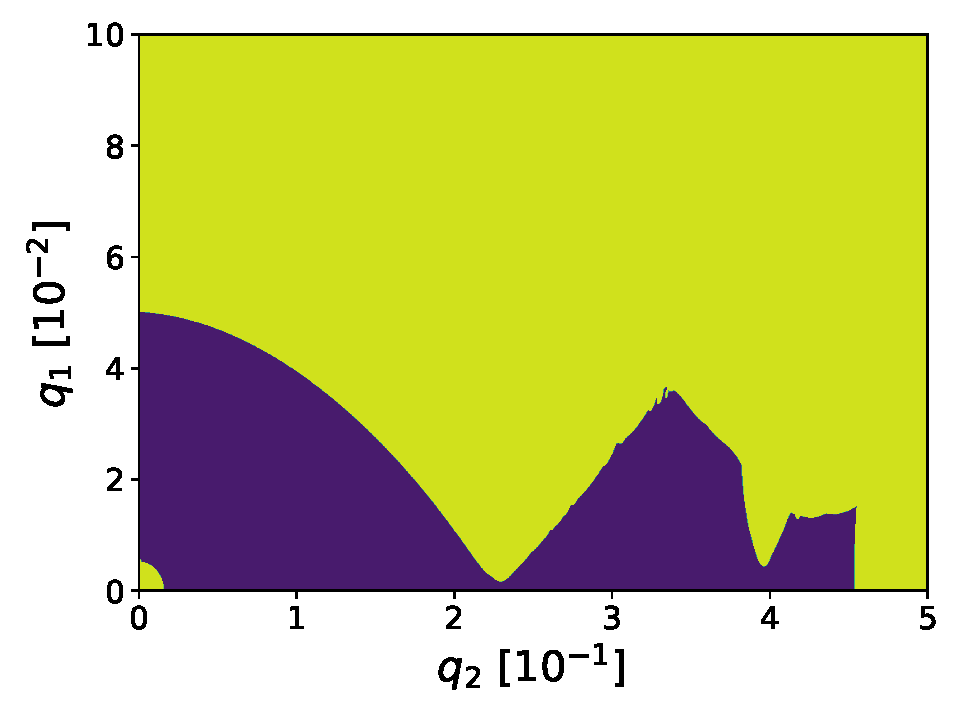
\includegraphics[width=\linewidth]{img/0_ions_1_electrons_q1_0.0-0.1_q2_0.0-0.5_960x960_3.pdf}  
  \caption{Simulation}
  \label{fig:sim_3}
\end{subfigure}
\caption{Stability diagrams for $\nicefrac{\Omega_2}{\Omega_1} = 3$}
\label{fig:stabil-eta=3}
\end{figure}

In the sub-figure \ref{fig:det_3} we can see stable\textit{(dark)} and unstable\textit{(light)} regions of the studied differential equation. The adjacent image shows the stability of an electron based on numerical simulation. In contrast with the determinant solution, we can see that the two stability areas have melted away in the field with higher amplitudes. We must not forget that the stability in the figure \ref{fig:det_3} is calculated only along the z-axis. We can investigate this by setting the initial position and velocity in x-y directions to zero. As we can see, the subsequent picture \ref{fig:sim_3_z-direction} already agrees with the determinant solution \ref{fig:det_3}.

\begin{figure}[H]
\begin{subfigure}{.5\textwidth}
  \centering
  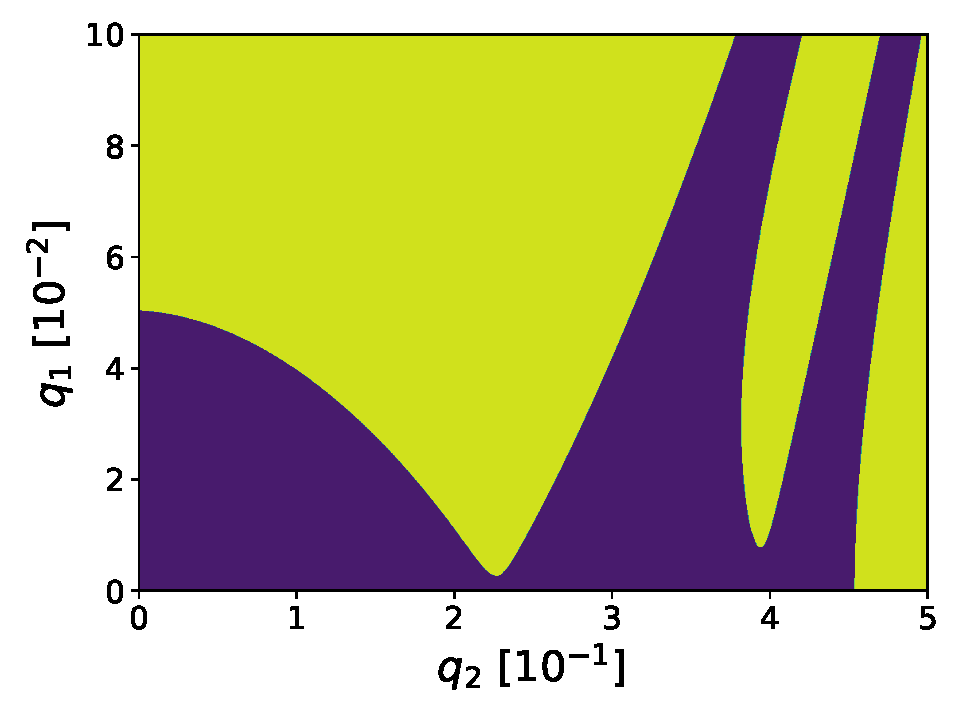
\includegraphics[width=\linewidth]{img/0_ions_1_electrons_q1_0.0-0.1_q2_0.0-0.5_992x992_3.pdf}
  \caption{Simulation in z-direction}
  \label{fig:sim_3_z-direction}
\end{subfigure}%
\begin{subfigure}{.5\textwidth}
  \centering
  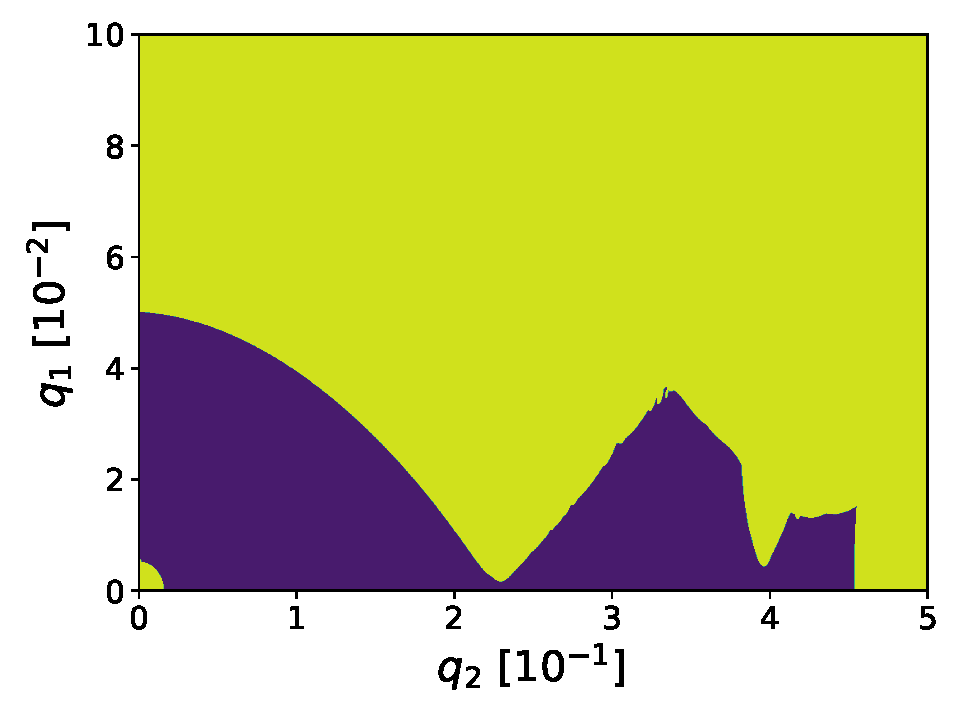
\includegraphics[width=\linewidth]{img/0_ions_1_electrons_q1_0.0-0.1_q2_0.0-0.5_960x960_3.pdf}  
  \caption{Simulation with x-y stability edge}
  \label{fig:sim_3_x-y_edge}
\end{subfigure}
\caption{Stability diagrams for $\nicefrac{\Omega_2}{\Omega_1} = 3$}
\label{fig:stabil-eta=3 different directions}
\end{figure}

In the next set of pictures \ref{fig:stabil-eta=3_x-y_directions}, we evaluate the stability diagram in x-y directions by setting $\zeta = x$ in \eqref{tilde params} for a determinant solution and setting the z-component of initial position and velocity to zero in the simulation. The contour plot \ref{fig:sim_3_x-y_edge} was created with the enhanced condition for identifying stable solutions from the standard \eqref{stability condition in simulation}: $\max\limits_{x \in \mathcal{L}}(r) \leq 0.8 \ \ell_0$ to $\max\limits_{x \in \mathcal{L}}(r) \leq 4 \ \ell_0$. The\todo{add the green line to this picture} \xxx{green} trace embodies the edge of stability made with our standard \eqref{stability condition in simulation} stability requirement in simulation. So this picture, among others, illustrates the non-equivalence of our condition and the condition for stability we use in Floquet theory, as we have already mentioned in \ref{foot:different stability condition}. The\todo{add the green line to this picture} \xxx{green} line in \ref{fig:sim_3_x-y_edge} represents the stability edge taken from \ref{fig:stabil-eta=3_x-y_directions}, explaining the difference between stability diagrams \ref{fig:stabil-eta=3}. We obtain an important closure that holds for all the other frequency ratios as well. The discrepancy between determinant and simulated stability diagrams is resolved by the necessity to combine determinant solutions in both x and z directions. This can be easily fixed with the cost of doubling the computation time for a determinant solution. Nonetheless, from now on, we will focus on simulated results, keeping the determinant diagrams in the z-direction for comparison. Moreover, we can use these pictures as our sanity check. By matching them with the results from \cite{leefer2017investigation} \textit{(where the stability of the ideal quadrupole trap along the x-direction was studied)}, we see that we have reproduced the same\footnote{Note that they have used different condition to identify stable solutions.} results $\rightarrow$ proving the validity of our code, at least to some extent.
\begin{figure}[H]
\begin{subfigure}{.5\textwidth}
  \centering
  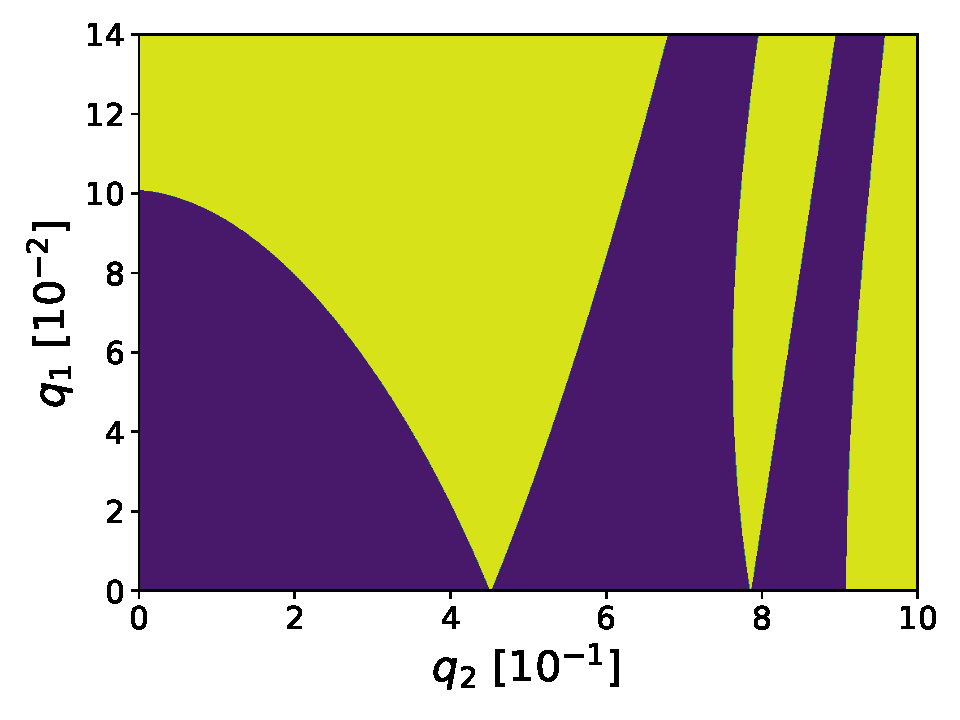
\includegraphics[width=\linewidth]{img/det_q1_0.0-0.14_q2_0.0-1.0_960x960_3.pdf}
  \caption{Determinant in x-direction}
  \label{fig:det_3_x-direction}
\end{subfigure}%
\begin{subfigure}{.5\textwidth}
  \centering
  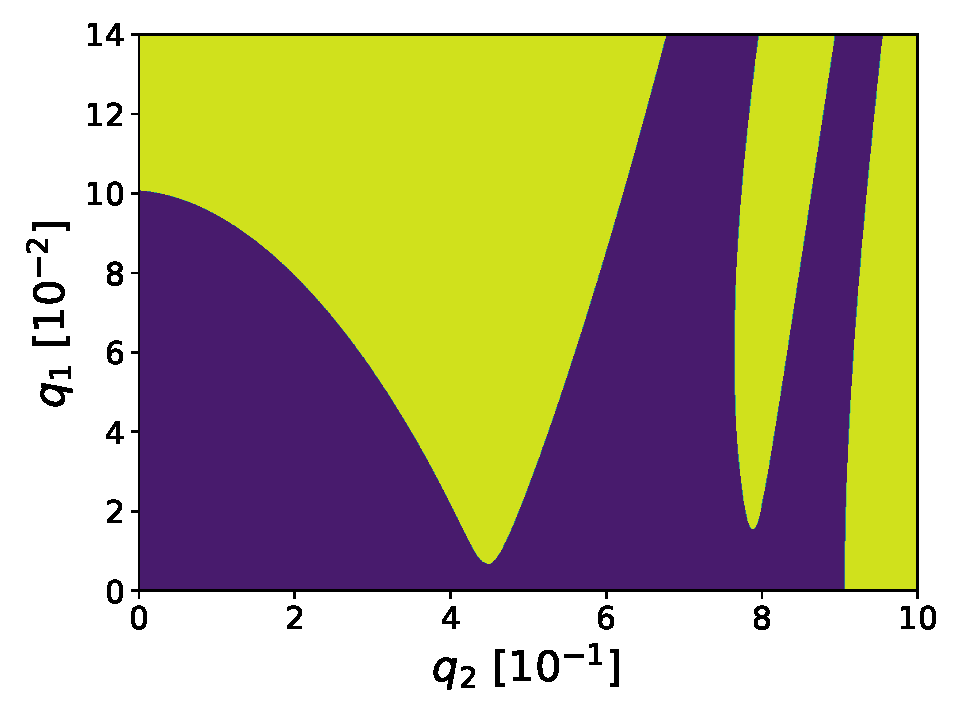
\includegraphics[width=\linewidth]{img/0_ions_1_electrons_q1_0.0-0.14_q2_0.0-1.0_984x984_3.pdf}  
  \caption{Simulation in x-y plane}
  \label{fig:sim_3_x-direction}
\end{subfigure}
\caption{Stability diagrams for $\nicefrac{\Omega_2}{\Omega_1} = 3$ in x-y plane}
\label{fig:stabil-eta=3_x-y_directions}
\end{figure} 
The image \ref{fig:velocityedge-eta=3} combines two pictures. The pink curve construes the stable regions simulated for the figure \ref{fig:sim_3}. In the background is a contour plot of the average electron velocity $\langle v \rangle$ throughout the whole trajectory\footnote{Average value defined as: $\langle \xi \rangle = \nicefrac{1}{T} \int_{0}^{T} \xi(\tau) \, d\tau,$ where $T$ denotes a total time of simulation.} relative to the initial velocity $v_0$. The color bar to the right indicates the value of this ratio. We create all the other figures similar to \ref{fig:velocityedge-eta=3} in the same way. These diagrams can help us find stable trap parameters while keeping electron temperature as low as possible, which is our ultimate goal.
\begin{figure}[H]
	\centering
	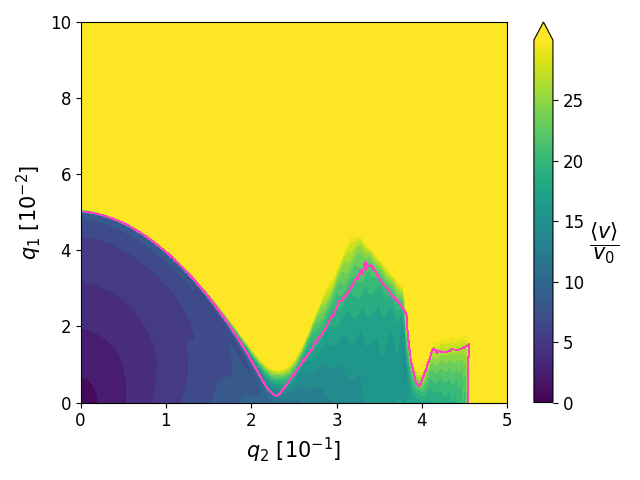
\includegraphics[width=\linewidth]{img/0_ions_1_electrons_q1_0.0-0.1_q2_0.0-0.5_960x960_3_1000.png}
	\caption{Average electron velocity for $\nicefrac{\Omega_2}{\Omega_1} = 3$}
	\label{fig:velocityedge-eta=3}
\end{figure}

Moving to larger frequency ratio $\rightarrow \nicefrac{\Omega_2}{\Omega_1} = 13$ we can start to notice some patterns.

\begin{figure}[H]
\begin{subfigure}{.5\textwidth}
  \centering
  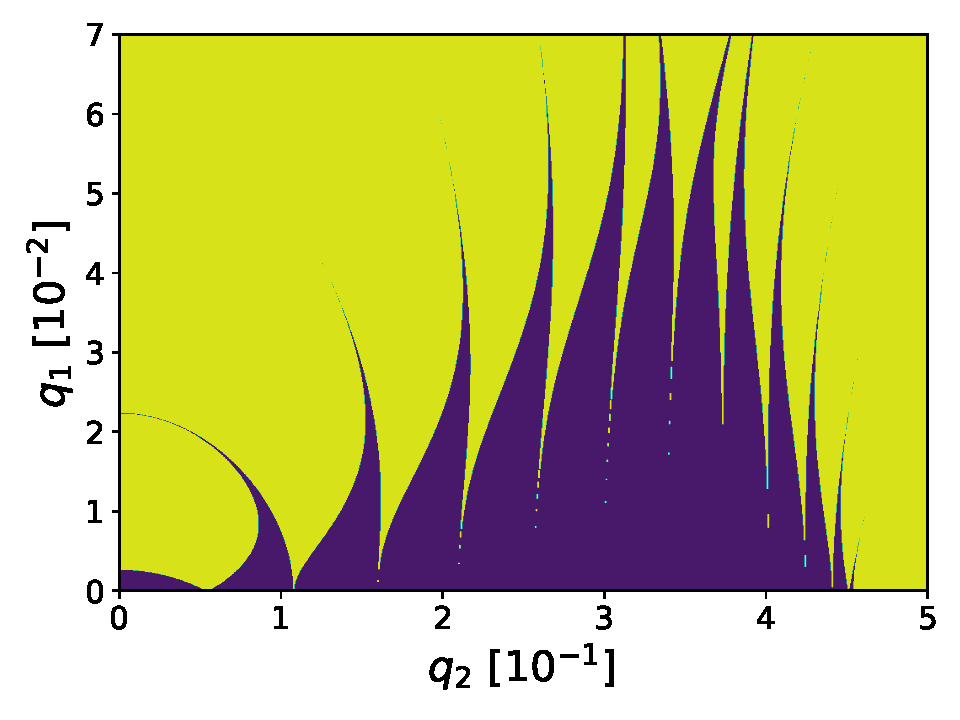
\includegraphics[width=\linewidth]{img/det_q1_0.0-0.07_q2_0.0-0.5_960x960_13.pdf}
  \caption{Determinant}
  \label{fig:det_13}
\end{subfigure}%
\begin{subfigure}{.5\textwidth}
  \centering
  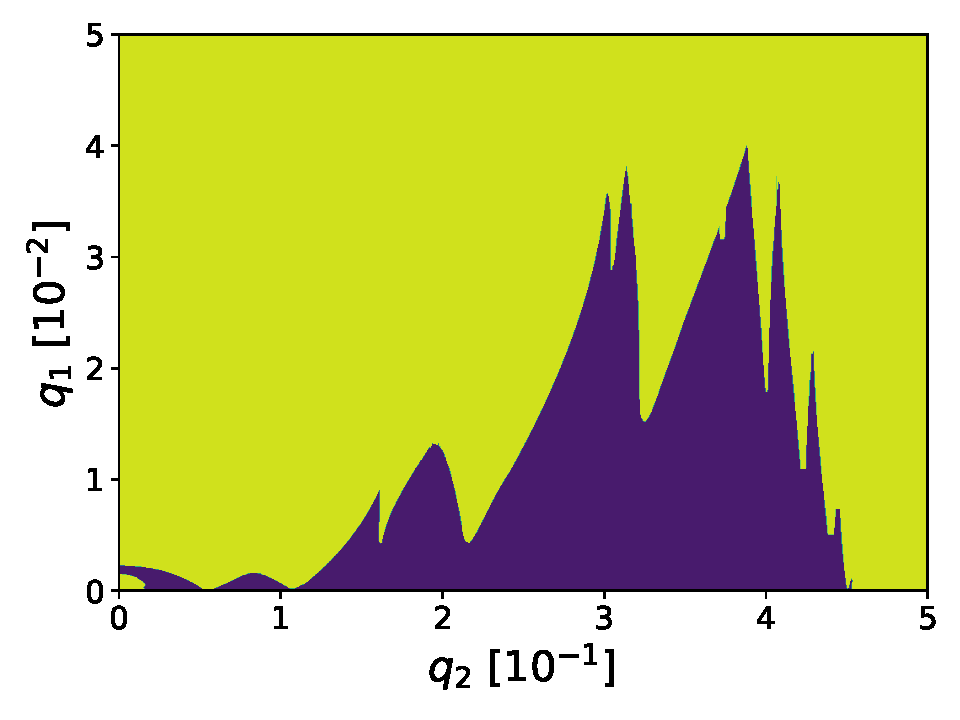
\includegraphics[width=\linewidth]{img/0_ions_1_electrons_q1_0.0-0.05_q2_0.0-0.5_960x960_13.pdf}  
  \caption{Simulation}
  \label{fig:sim_13}
\end{subfigure}
\caption{Stability diagrams for $\nicefrac{\Omega_2}{\Omega_1} = 13$}
\label{fig:velocityedge-eta=13}
\end{figure}

\begin{figure}[H]
	\centering
	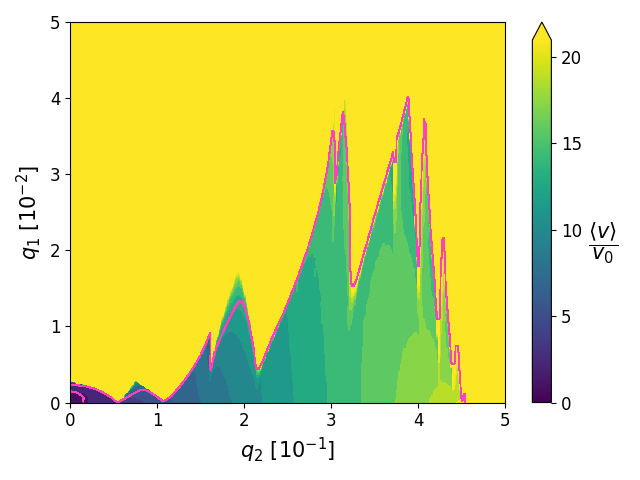
\includegraphics[width=\linewidth]{img/0_ions_1_electrons_q1_0.0-0.05_q2_0.0-0.5_960x960_13_1000.png}
	\caption{Average electron velocity for $\nicefrac{\Omega_2}{\Omega_1} = 13$}
	\label{fig:stabil-eta=13}
\end{figure}

There emerges one stable triangle with many tongues of instability. With an increasing ratio $\nicefrac{\Omega_2}{\Omega_1}$ we can see a gain in the number of these tongues, but their width promptly shrinks as well. We expect that by further increasing the frequency ratio, the unstable tongues will be realistically affecting only the regions near the edge of stability, leaving the regions further inside a stable triangle safe to work with.

\xxx{Continuing to the frequency ratio compatible for trapping electrons and Ca+ ions}

\begin{figure}[H]
\begin{subfigure}{.5\textwidth}
  \centering
  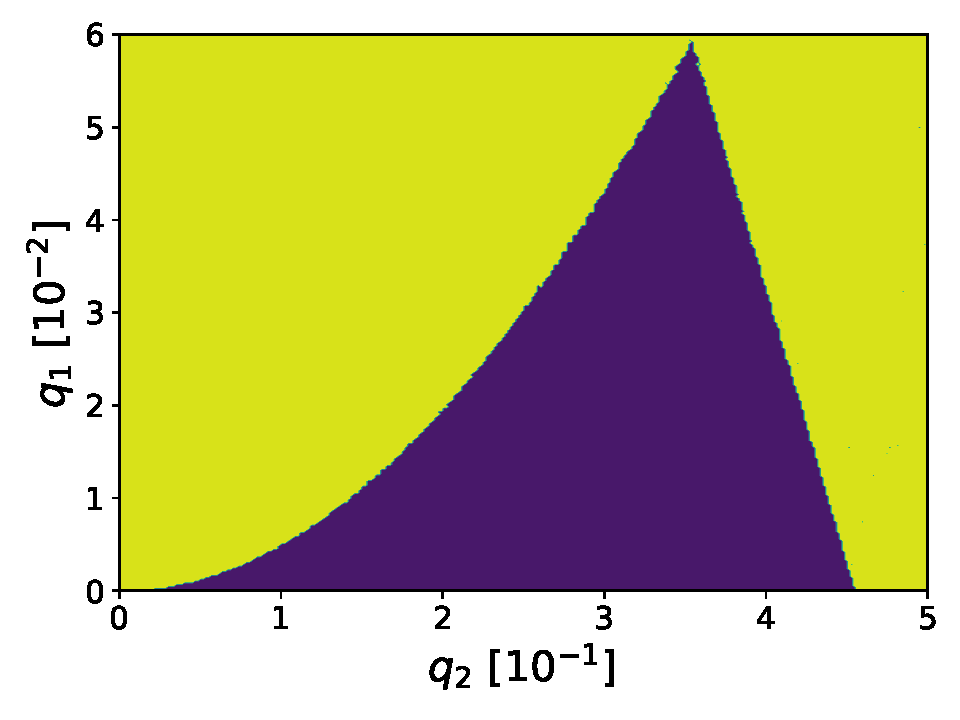
\includegraphics[width=\linewidth]{img/det_q1_0.0-0.06_q2_0.0-0.5_300x300_833.pdf}
  \caption{Determinant}
  \label{fig:det_833}
\end{subfigure}%
\begin{subfigure}{.5\textwidth}
  \centering
  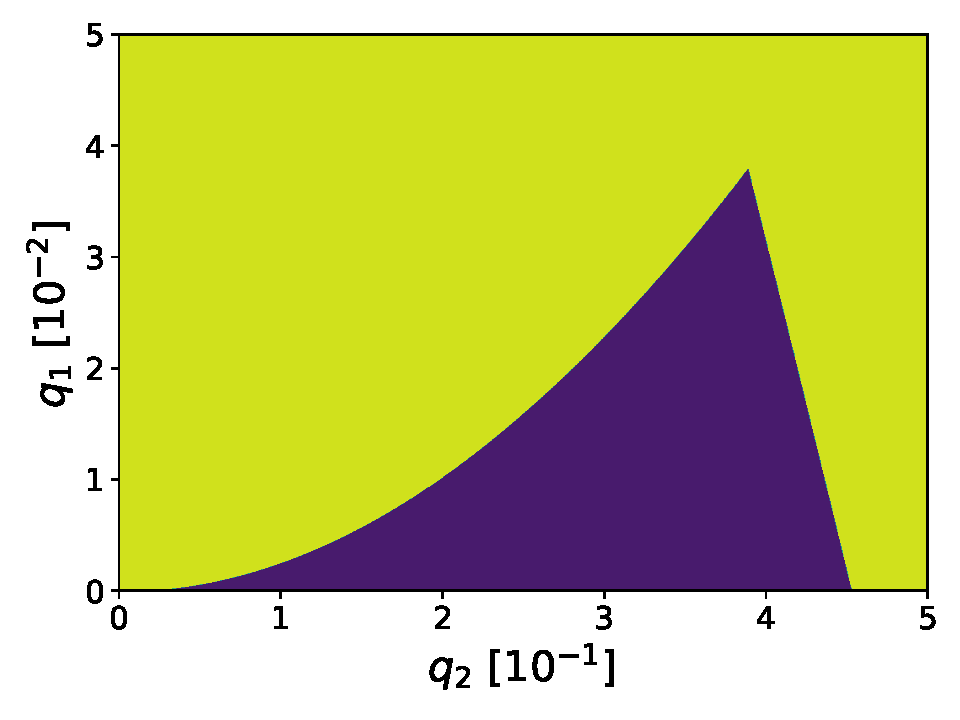
\includegraphics[width=\linewidth]{img/0_ions_1_electrons_q1_0.0-0.05_q2_0.0-0.5_960x960_833.pdf}  
  \caption{Simulation}
  \label{fig:sim_833}
\end{subfigure}
\caption{Stability diagrams for $\nicefrac{\Omega_2}{\Omega_1} = 833$}
\label{fig:stabil-eta=833}
\end{figure}

It is worth pointing out that the computation time of the determinant stability diagram already exceeds that of simulated for this frequency ratio. Nevertheless, we apply a built-in NumPy\footnote{NumPy is widely used, open source, numerical python library: \href{https://numpy.org}{https://numpy.org/}} function for computing determinants using LU decomposition \cite{teukolsky1992numerical} with time complexity $\mathcal{O}(n^3)$, not utilizing the fact that our matrices are sparse. Moreover, we are interested only in the sign of a determinant which also suggests a capacity for efficiency improvement. But since the determinant solutions are not essential to us, we do not investigate such further advancements in this thesis.

\begin{figure}[H]
	\centering
	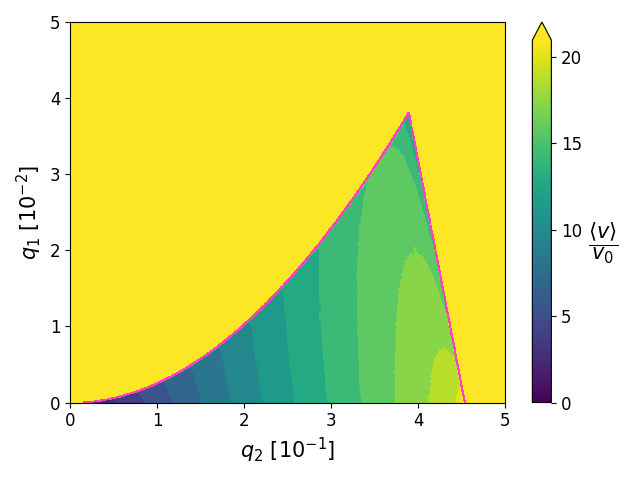
\includegraphics[width=\linewidth]{img/0_ions_1_electrons_q1_0.0-0.05_q2_0.0-0.5_960x960_833_1000.png}
	\caption{Simulated stability diagram for $\nicefrac{\Omega_2}{\Omega_1} = 833$}
	\label{fig:stabil-eta=833}
\end{figure}

\subsection{Dependence on initial conditions}

\xxx{work in progress\dots}

\begin{figure}[H]
\begin{subfigure}{.3\textwidth}
  \centering
  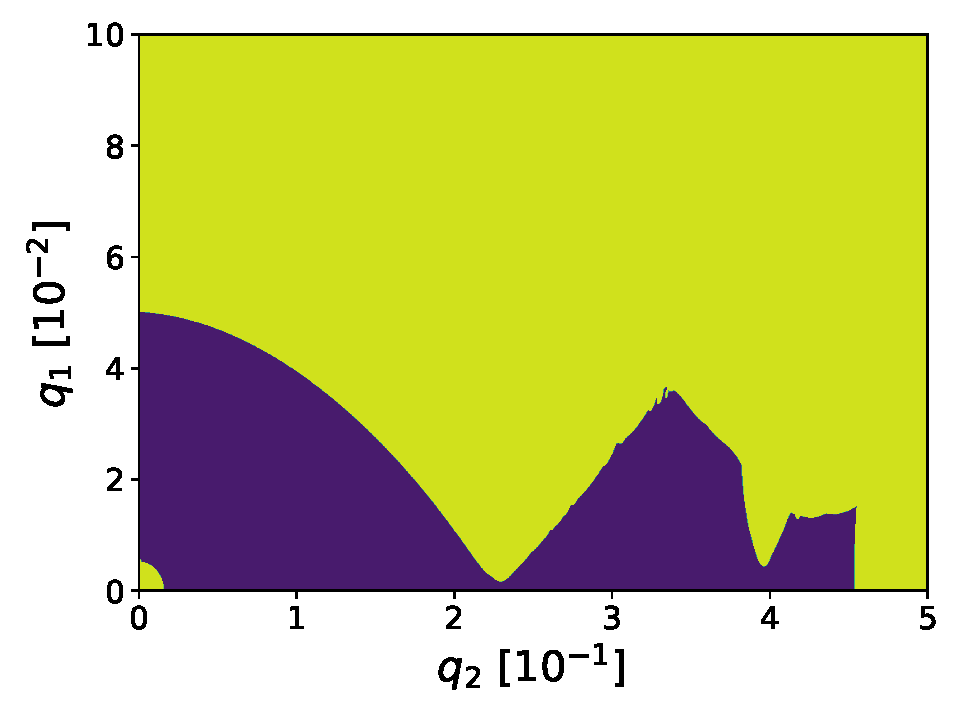
\includegraphics[width=\linewidth]{img/0_ions_1_electrons_q1_0.0-0.1_q2_0.0-0.5_960x960_3.pdf}
  \caption{Normal initial conditions}
  \label{fig:normal_conds-3}
\end{subfigure}%
\begin{subfigure}{.3\textwidth}
  \centering
  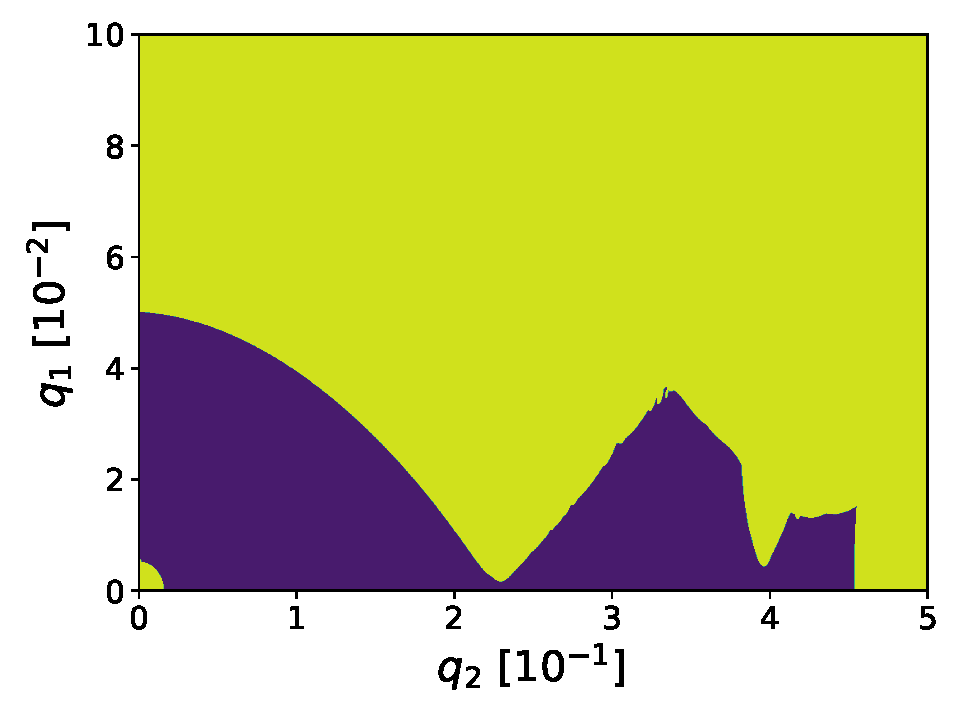
\includegraphics[width=\linewidth]{img/0_ions_1_electrons_q1_0.0-0.1_q2_0.0-0.5_960x960_3.pdf}
  \caption{High velocity}
  \label{fig:high_velocity-3}
\end{subfigure}%
\begin{subfigure}{.3\textwidth}
  \centering
  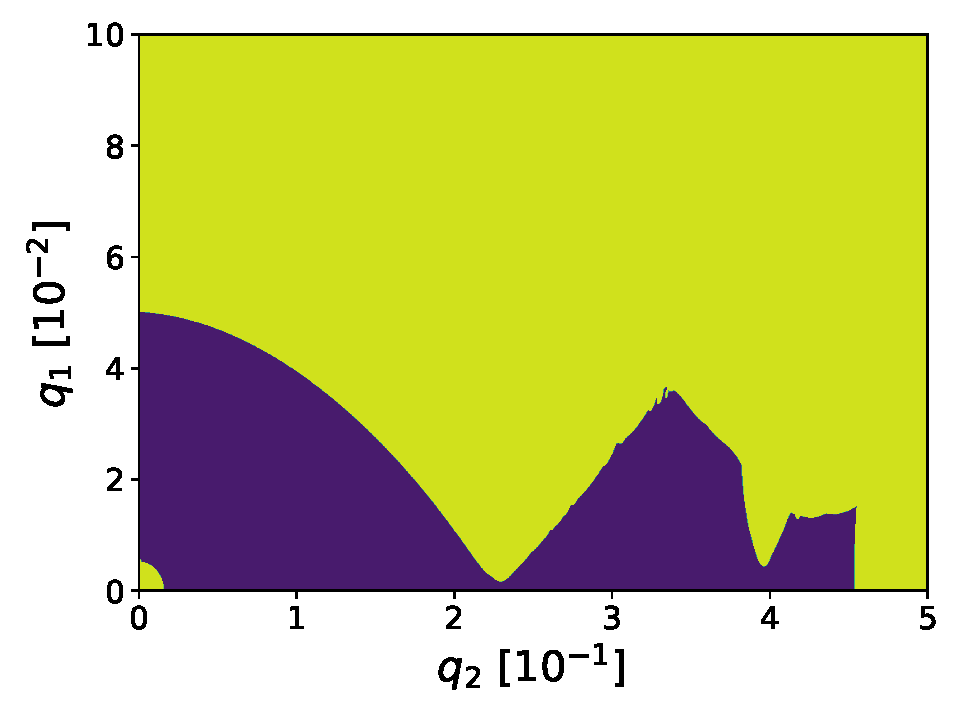
\includegraphics[width=\linewidth]{img/0_ions_1_electrons_q1_0.0-0.1_q2_0.0-0.5_960x960_3.pdf}  
  \caption{Further away from center}
  \label{fig:large_radius-3}
\end{subfigure}
\caption{$\nicefrac{\Omega_2}{\Omega_1} = 3$, different initial conditions}
\label{fig:init-conds-eta=3}
\end{figure}

High initial velocity \ref{fig:high_velocity-3} makes the region with the weakest field (around $q_1 \approx q_2 \approx 0$) unstable, which is understandable since the stability condition \xxx{reference} is not satisfied. A wider distance from the trap's center combined with the initial velocity pointing away from the trap \ref{fig:large_radius-3} distorts the stability diagram's shape significantly. 

\xxx{as a sanity check we try to reproduce a result from \cite{leefer2017investigation}.} 

\section{Creating a Coulomb crystal}
\xxx{currently making some useable pictures}

\section{Stability of electron in Coulomb crystal}
\subsection{One electron - one ion}
\subsection{One electron - twenty ions}
\subsection{One electron - a hundred ions}

\section{Design of the experiment}

\section{Future}
\label{chap:future}

Our concerns in the future will be reproducing results of this thesis for the real planar geometry of the trap used in our experiment. The potential of such a trap can be formulated in integral form utilizing Bessel functions, which will make our simulations much more computationally expensive. We need to derive equation of motion and identify parameters analogous to $a$, $q_1$ and $q_2$ which we had for ideal quadrupole trap. After that we can use our exiting program to study stability of particles in dependence on such parameters exactly as we did in this thesis. 